\section{More Information}
\label{sec:more-info}

\subsection{Contacts}
Peter Ascoli and Jackie Song can be contacted through their personal sites, \url{http://peterascoli.com/} and \url{http://jsong.me/} respectively. Professor Wei can be reached through his Cooper Union faculty web page, \url{http://www.cooper.edu/engineering/people/chih-shing-wei}. 

\subsection{Repositories}
The \LaTeX\ source for this report is available at \url{https://github.com/songjx/carbon-fiber}. The Marlin configuration for this project is available at \url{https://github.com/songjx/Marlin}. 

\subsection{FANUC}
To obtain PDFs of the referenced manuals for the FANUC equipment described in this report, contact JackieSong, Peter Ascoli, or Professor Wei. For spare parts, tech support, and repairs, make an account at the FANUC America cRc Online Site at \url{https://crc.frc.com/main.aspx}. The FANUC-provided F number is required to sign up; the new account will have access to all previous support tickets. The F number is printed on several labels on the controller and robot, pictured in Figure~\ref{fig:f-no}. Some other FANUC equipment identification labels are shown in Figure~\ref{fig:stickers}.  

\begin{figure}
    \centering
    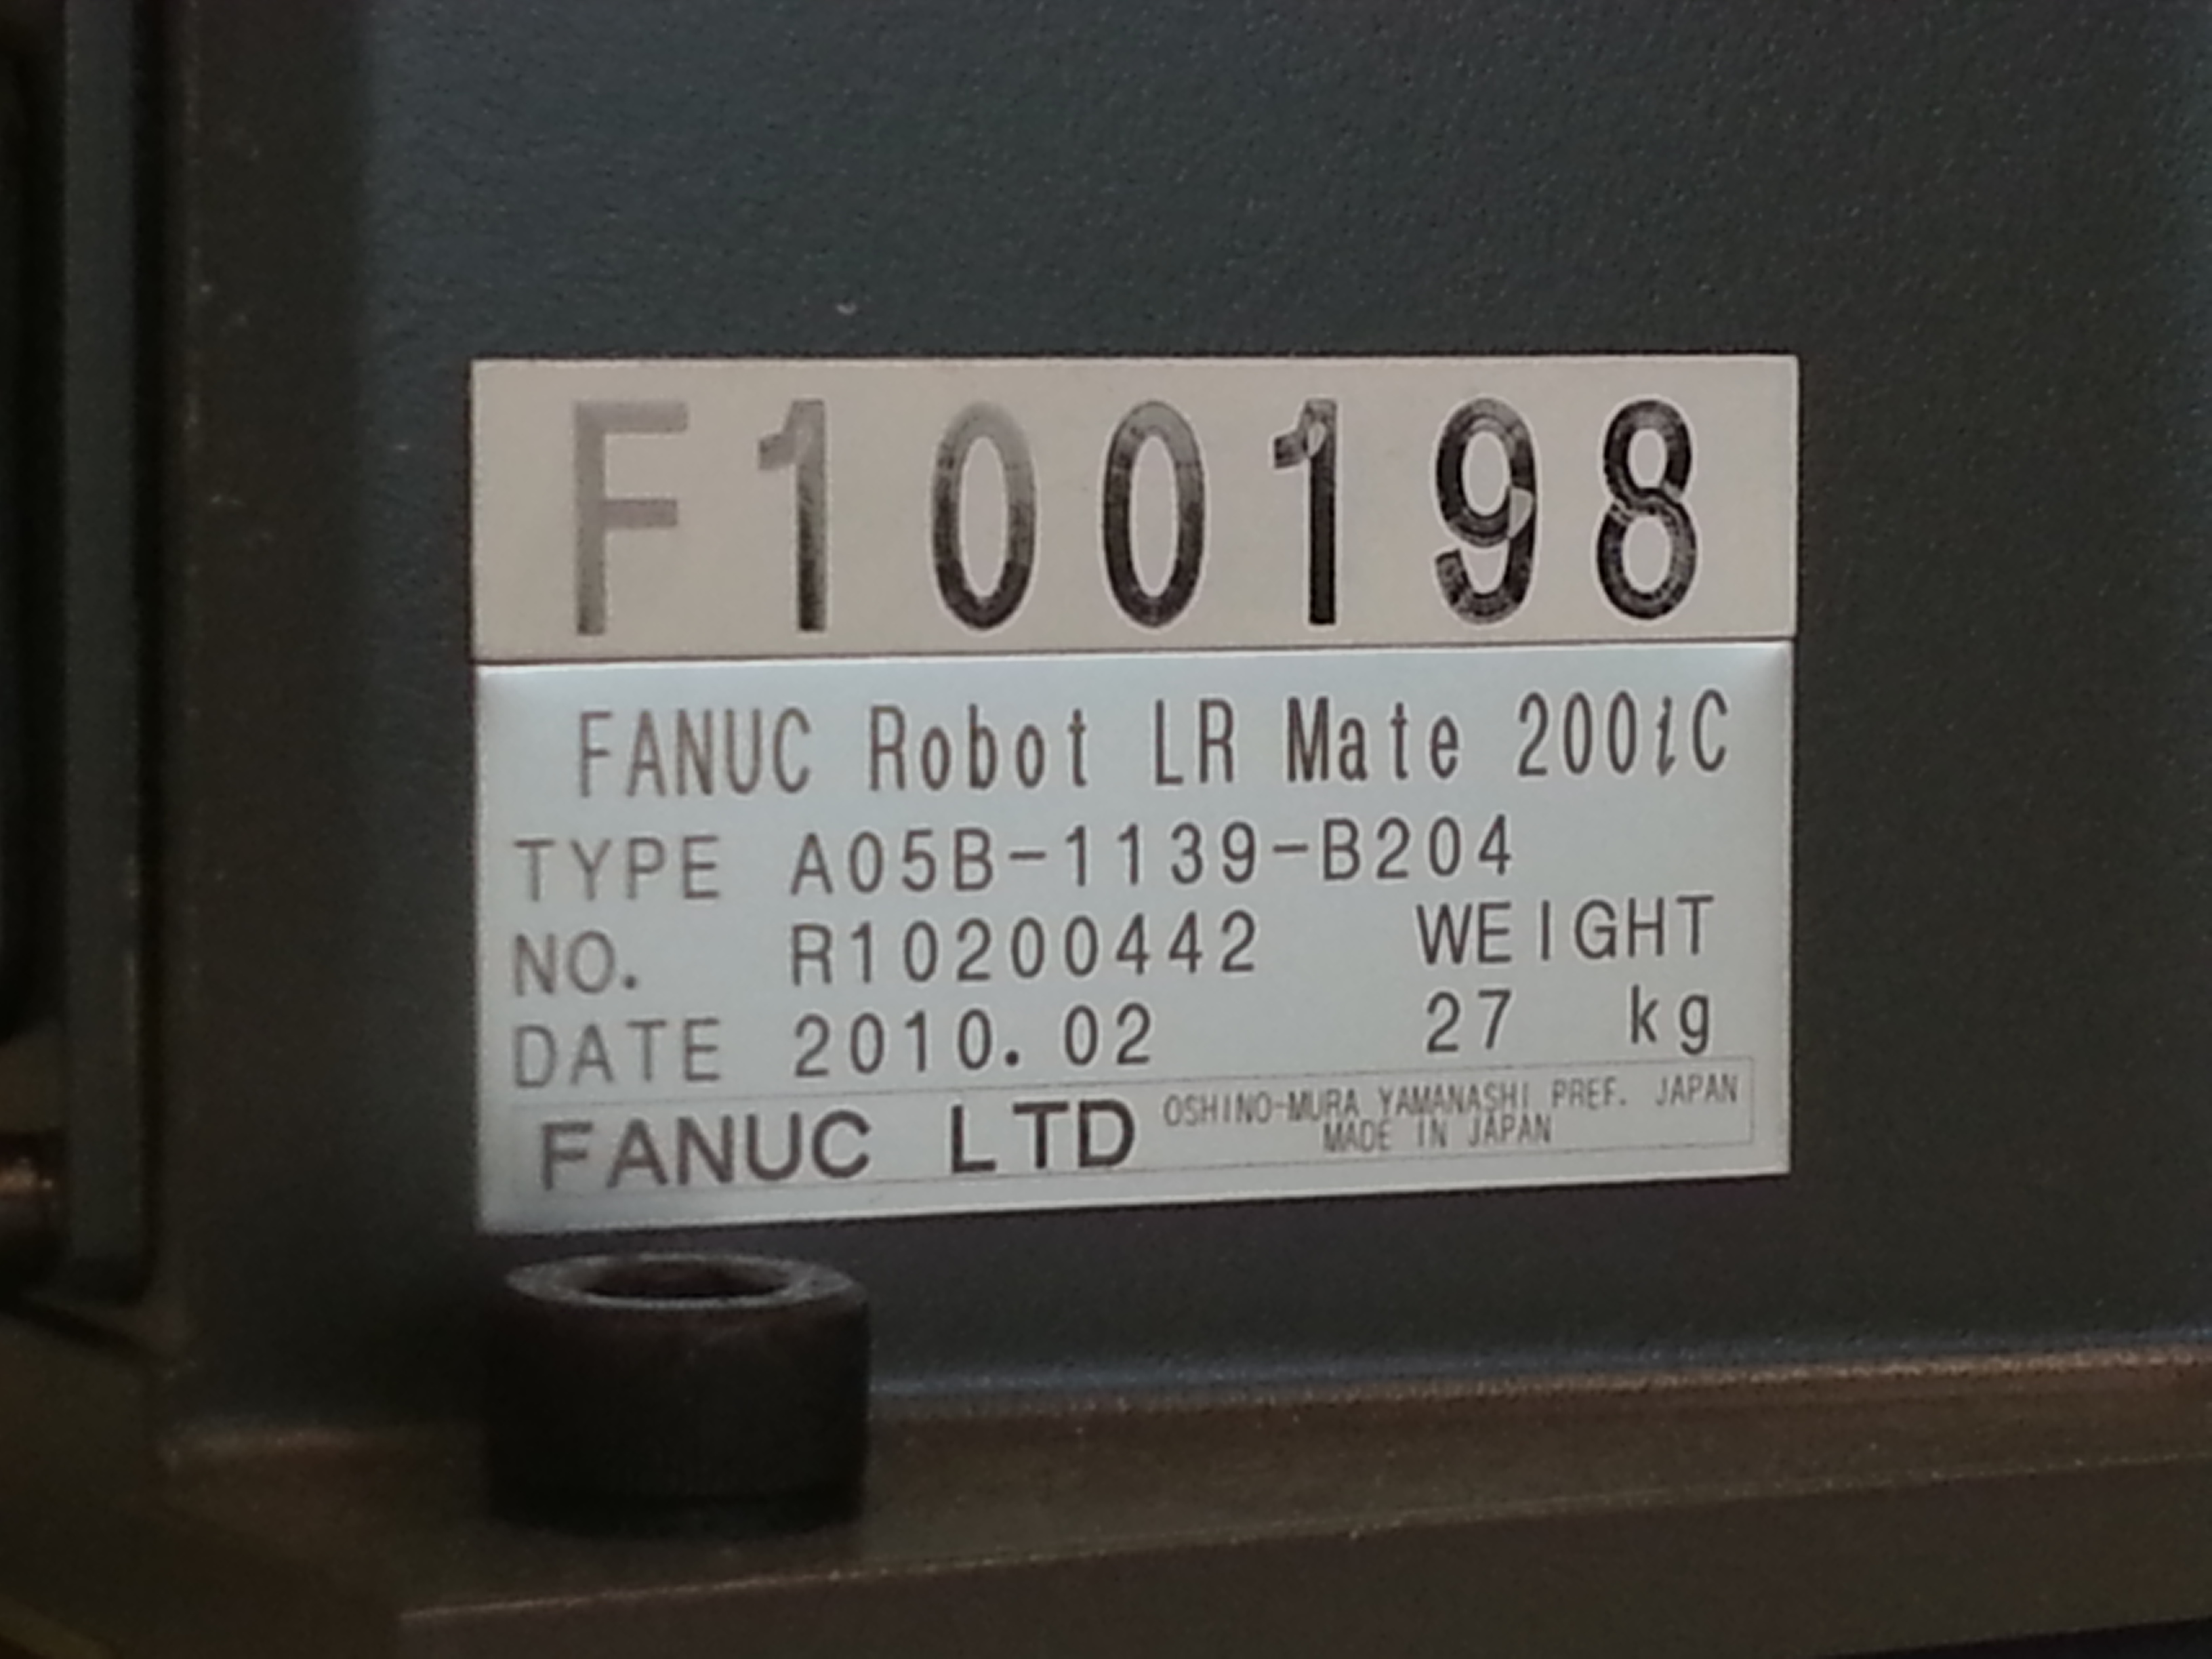
\includegraphics[width=.4\linewidth]{figures/stickers/f-no}
    \caption{Robot F number label.}
    \label{fig:f-no}
\end{figure}

\begin{figure}
    \centering
    \begin{subfigure}{.5\textwidth}
        \centering
        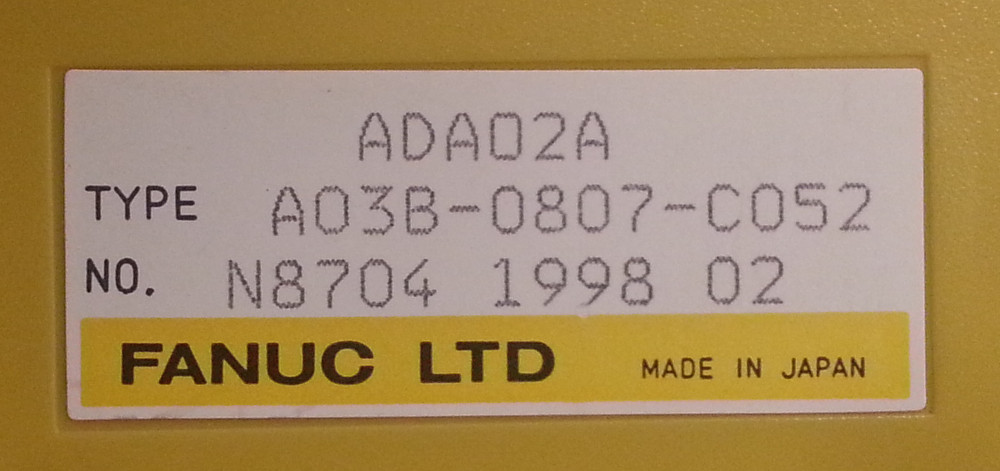
\includegraphics[width=.8\linewidth]{figures/stickers/ao}
    \end{subfigure}%
    \begin{subfigure}{.5\textwidth}
        \centering
        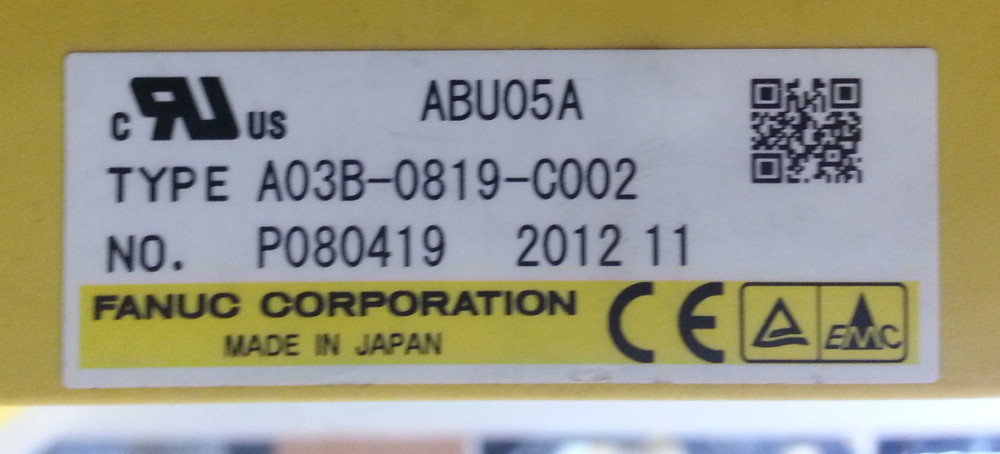
\includegraphics[width=.8\linewidth]{figures/stickers/backplane}
    \end{subfigure} \\
    \begin{subfigure}{.5\textwidth}
        \centering
        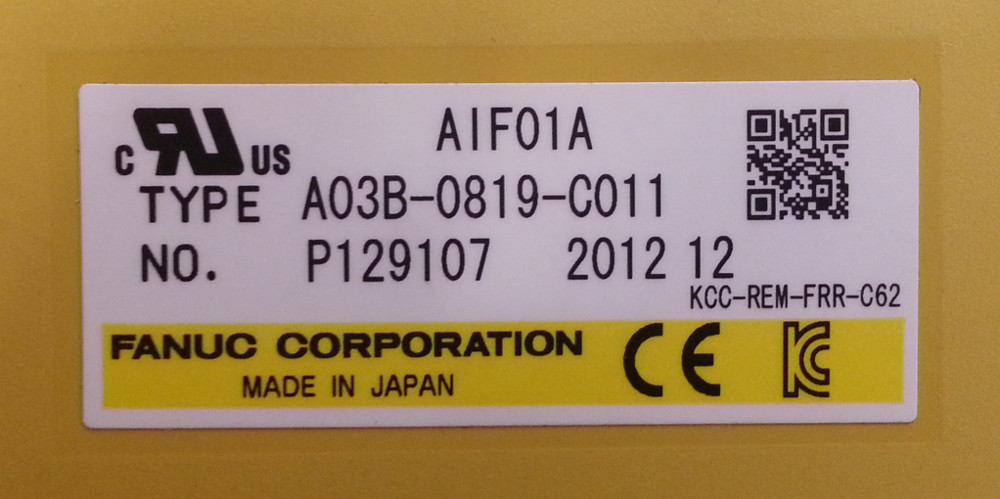
\includegraphics[width=.8\linewidth]{figures/stickers/io-unit}
    \end{subfigure}%
    \begin{subfigure}{.5\textwidth}
        \centering
        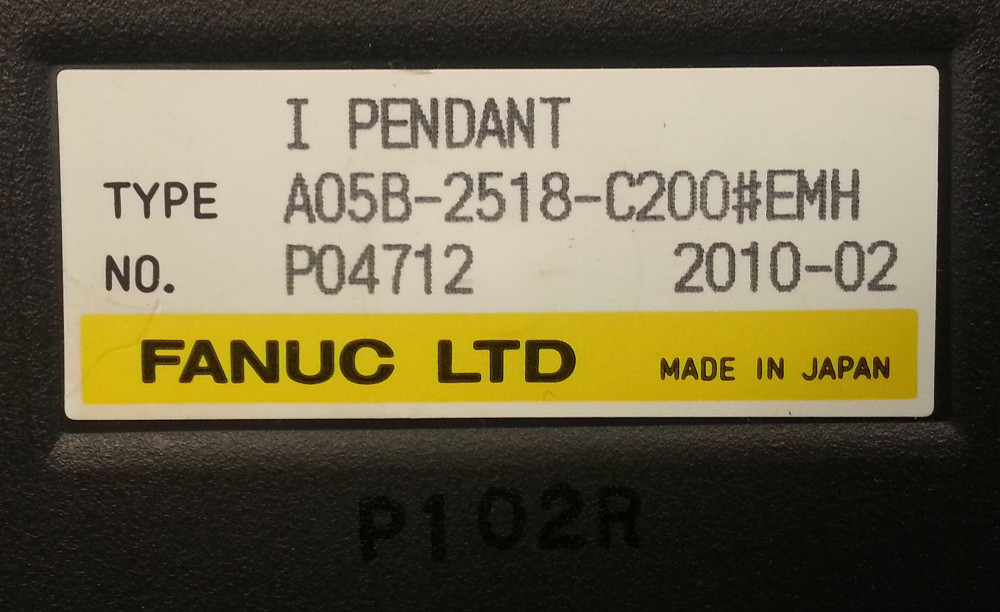
\includegraphics[width=.8\linewidth]{figures/stickers/tp}
    \end{subfigure} \\
    \begin{subfigure}{.5\textwidth}
        \centering
        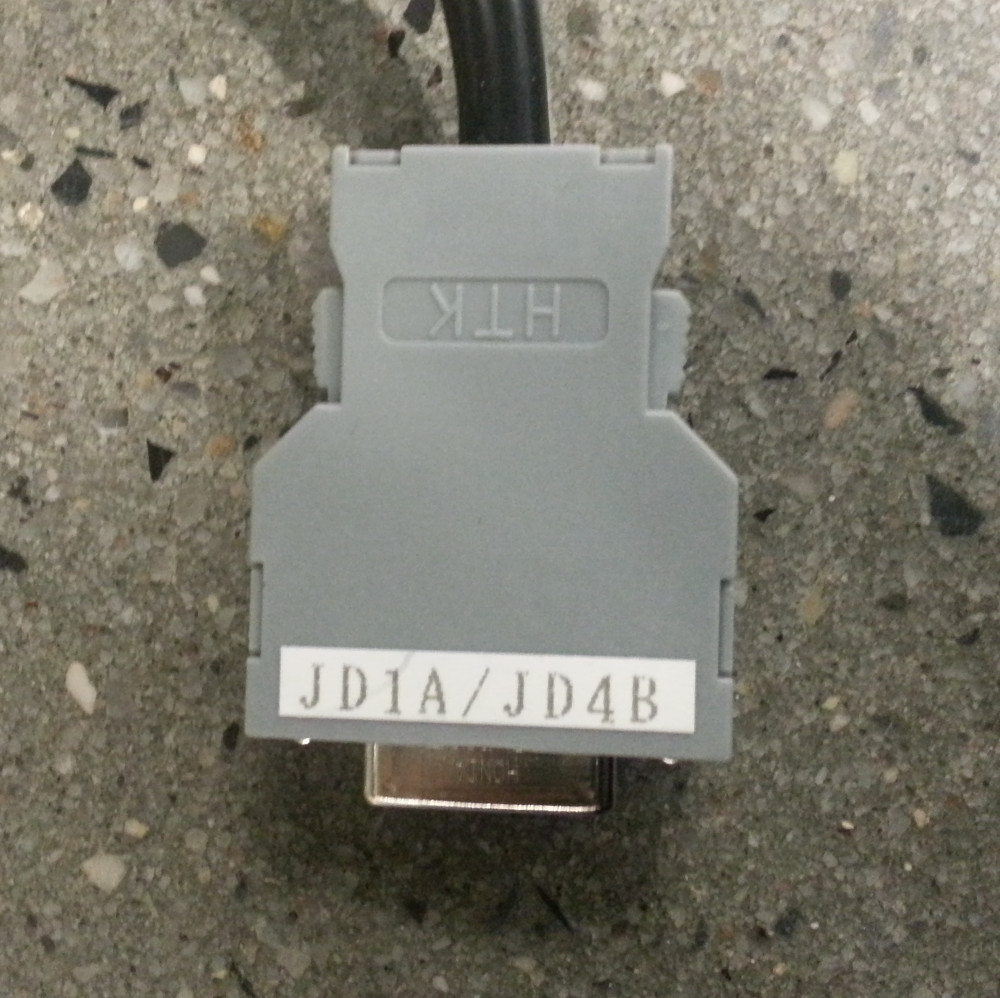
\includegraphics[width=.8\linewidth]{figures/stickers/io-link-a-connector}
    \end{subfigure}%
    \begin{subfigure}{.5\textwidth}
        \centering
        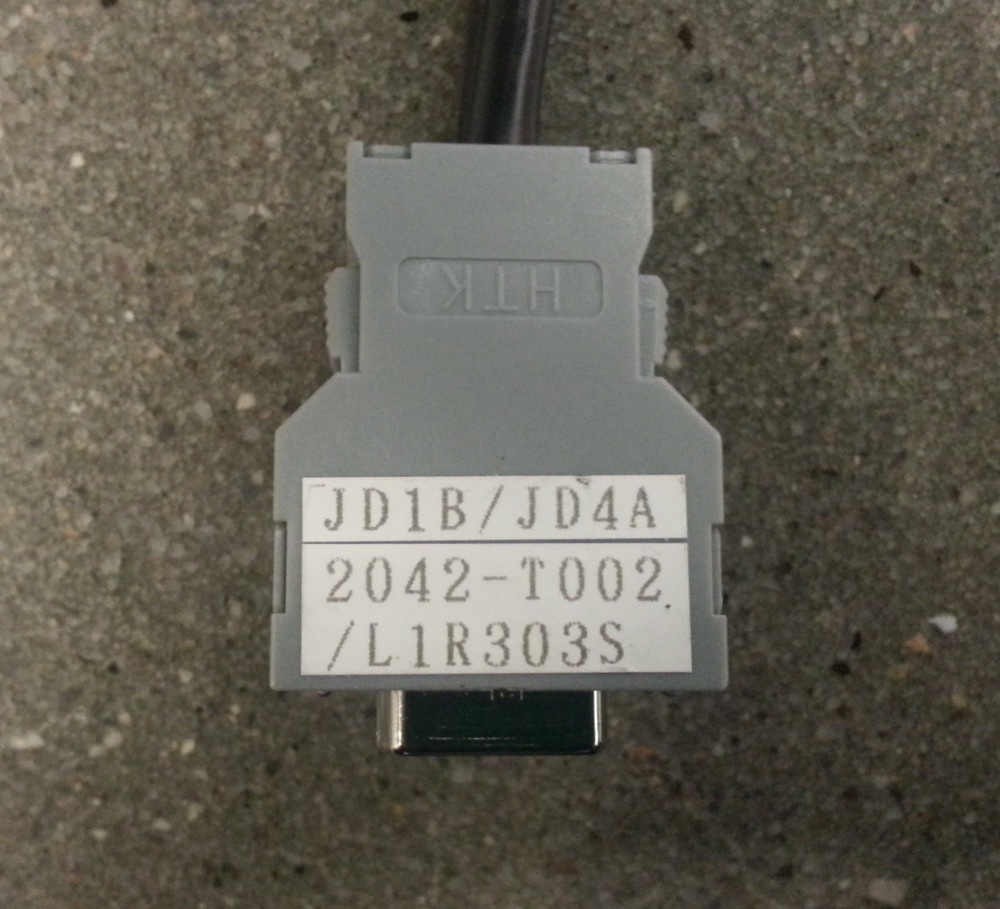
\includegraphics[width=.8\linewidth]{figures/stickers/io-link-b-connector}
    \end{subfigure}
    \caption{More FANUC equipment identification labels.}
    \label{fig:stickers}
\end{figure}

\subsection{CAD}
CAD files for this project can be obtained by contacting Peter Ascoli or Jackie Song.

\subsection{FEA}
FEA files for this project can be obtained by contacting Peter Ascoli or Jackie Song.

\subsection{Software}
Schematics in this report were generated using several software packages, including draw.io, ExpressSCH, Adobe Illustrator, and Inkscape. Git was used for version control. The Arduino IDE was used to compile and upload the Marlin firmware. \LaTeX\ was used to generate this report. SolidWorks and AutoCAD were used to create CAD models and drawings. 
